\documentclass[14pt,russian]{scrartcl}
\let\counterwithout\relax
\let\counterwithin\relax
\usepackage{lmodern}
\usepackage{float}
\usepackage{xcolor}
\usepackage{extsizes}
\usepackage{subfig}
\usepackage[export]{adjustbox}
\usepackage{tocvsec2} % возможность менять учитываемую глубину разделов в оглавлении
\usepackage[subfigure]{tocloft}

\usepackage{fancyvrb}
\usepackage{ulem,bm,mathrsfs,ifsym} %зачеркивания, особо жирный стиль и RSFS начертание
\usepackage{sectsty} % переопределение стилей подразделов
%%%%%%%%%%%%%%%%%%%%%%%

%%% Поля и разметка страницы %%%
\usepackage{pdflscape}                              % Для включения альбомных страниц
\usepackage{geometry}                               % Для последующего задания полей
\geometry{a4paper,tmargin=2cm,bmargin=2cm,lmargin=3cm,rmargin=1cm} % тоже самое, но лучше

%%% Математические пакеты %%%
\usepackage{amsthm,amsfonts,amsmath,amssymb,amscd}  % Математические дополнения от AMS
\usepackage{mathtools}                              % Добавляет окружение multlined
\usepackage[perpage]{footmisc}

%%%% Установки для размера шрифта 14 pt %%%%
%% Формирование переменных и констант для сравнения (один раз для всех подключаемых файлов)%%
%% должно располагаться до вызова пакета fontspec или polyglossia, потому что они сбивают его работу
%\newlength{\curtextsize}
%\newlength{\bigtextsize}
%\setlength{\bigtextsize}{13pt}
\KOMAoptions{fontsize=14pt}

\makeatletter
\def\showfontsize{\f@size{} point}
\makeatother

%\makeatletter
%\show\f@size                                       % неплохо для отслеживания, но вызывает стопорение процесса, если документ компилируется без команды  -interaction=nonstopmode 
%\setlength{\curtextsize}{\f@size pt}
%\makeatother

%шрифт times
\usepackage{tempora}

   %%% Решение проблемы копирования текста в буфер кракозябрами
%    \input glyphtounicode.tex
%    \input glyphtounicode-cmr.tex %from pdfx package
%    \pdfgentounicode=1
    \usepackage{cmap}                               % Улучшенный поиск русских слов в полученном pdf-файле
    \usepackage[T2A]{fontenc}                       % Поддержка русских букв
    \usepackage[utf8]{inputenc}                     % Кодировка utf8
    \usepackage[english, main=russian]{babel}            % Языки: русский, английский
%   \IfFileExists{pscyr.sty}{\usepackage{pscyr}}{}  % Красивые русские шрифты
%\renewcommand{\rmdefault}{ftm}
%%% Оформление абзацев %%%
\usepackage{indentfirst}                            % Красная строка
%\usepackage{eskdpz}

%%% Таблицы %%%
\usepackage{longtable}                              % Длинные таблицы
\usepackage{multirow,makecell,array}                % Улучшенное форматирование таблиц
\usepackage{booktabs}                               % Возможность оформления таблиц в классическом книжном стиле (при правильном использовании не противоречит ГОСТ)

%%% Общее форматирование
\usepackage{soulutf8}                               % Поддержка переносоустойчивых подчёркиваний и зачёркиваний
\usepackage{icomma}                                 % Запятая в десятичных дробях



%%% Изображения %%%
\usepackage{graphicx}                               % Подключаем пакет работы с графикой
\usepackage{wrapfig}

%%% Списки %%%
\usepackage{enumitem}

%%% Подписи %%%
\usepackage{caption}                                % Для управления подписями (рисунков и таблиц) % Может управлять номерами рисунков и таблиц с caption %Иногда может управлять заголовками в списках рисунков и таблиц
%% Использование:
%\begin{table}[h!]\ContinuedFloat - чтобы не переключать счетчик
%\captionsetup{labelformat=continued}% должен стоять до самого caption
%\caption{}
% либо ручками \caption*{Продолжение таблицы~\ref{...}.} :)

%%% Интервалы %%%

%%% Счётчики %%%
\usepackage[figure,table,section]{totalcount}               % Счётчик рисунков и таблиц
\DeclareTotalCounter{lstlisting}
\usepackage{totcount}                               % Пакет создания счётчиков на основе последнего номера подсчитываемого элемента (может требовать дважды компилировать документ)
\usepackage{totpages}                               % Счётчик страниц, совместимый с hyperref (ссылается на номер последней страницы). Желательно ставить последним пакетом в преамбуле

%%% Продвинутое управление групповыми ссылками (пока только формулами) %%%
%% Кодировки и шрифты %%%

%   \newfontfamily{\cyrillicfont}{Times New Roman}
%   \newfontfamily{\cyrillicfonttt}{CMU Typewriter Text}
	%\setmainfont{Times New Roman}
	%\newfontfamily\cyrillicfont{Times New Roman}
	%\setsansfont{Times New Roman}                    %% задаёт шрифт без засечек
%	\setmonofont{Liberation Mono}               %% задаёт моноширинный шрифт
 %   \IfFileExists{pscyr.sty}{\renewcommand{\rmdefault}{ftm}}{}
%%% Интервалы %%%
%linespread-реализация ближе к реализации полуторного интервала в ворде.
%setspace реализация заточена под шрифты 10, 11, 12pt, под остальные кегли хуже, но всё же ближе к типографской классике. 
\linespread{1.3}                    % Полуторный интервал (ГОСТ Р 7.0.11-2011, 5.3.6)
%\renewcommand{\@biblabel}[1]{#1}

%%% Гиперссылки %%%
\usepackage{hyperref}

%%% Выравнивание и переносы %%%
\sloppy                             % Избавляемся от переполнений
\clubpenalty=10000                  % Запрещаем разрыв страницы после первой строки абзаца
\widowpenalty=10000                 % Запрещаем разрыв страницы после последней строки абзаца

\makeatletter % малые заглавные, small caps shape
\let\@@scshape=\scshape
\renewcommand{\scshape}{%
  \ifnum\strcmp{\f@series}{bx}=\z@
    \usefont{T1}{cmr}{bx}{sc}%
  \else
    \ifnum\strcmp{\f@shape}{it}=\z@
      \fontshape{scsl}\selectfont
    \else
      \@@scshape
    \fi
  \fi}
\makeatother

%%% Подписи %%%
%\captionsetup{%
%singlelinecheck=off,                % Многострочные подписи, например у таблиц
%skip=2pt,                           % Вертикальная отбивка между подписью и содержимым рисунка или таблицы определяется ключом
%justification=centering,            % Центрирование подписей, заданных командой \caption
%}
%%%        Подключение пакетов                 %%%
\usepackage{ifthen}                 % добавляет ifthenelse
%%% Инициализирование переменных, не трогать!  %%%
\newcounter{intvl}
\newcounter{otstup}
\newcounter{contnumeq}
\newcounter{contnumfig}
\newcounter{contnumtab}
\newcounter{pgnum}
\newcounter{bibliosel}
\newcounter{chapstyle}
\newcounter{headingdelim}
\newcounter{headingalign}
\newcounter{headingsize}
\newcounter{tabcap}
\newcounter{tablaba}
\newcounter{tabtita}
%%%%%%%%%%%%%%%%%%%%%%%%%%%%%%%%%%%%%%%%%%%%%%%%%%

%%% Область упрощённого управления оформлением %%%

%% Интервал между заголовками и между заголовком и текстом
% Заголовки отделяют от текста сверху и снизу тремя интервалами (ГОСТ Р 7.0.11-2011, 5.3.5)
\setcounter{intvl}{3}               % Коэффициент кратности к размеру шрифта

%% Отступы у заголовков в тексте
\setcounter{otstup}{0}              % 0 --- без отступа; 1 --- абзацный отступ

%% Нумерация формул, таблиц и рисунков
\setcounter{contnumeq}{1}           % Нумерация формул: 0 --- пораздельно (во введении подряд, без номера раздела); 1 --- сквозная нумерация по всей диссертации
\setcounter{contnumfig}{1}          % Нумерация рисунков: 0 --- пораздельно (во введении подряд, без номера раздела); 1 --- сквозная нумерация по всей диссертации
\setcounter{contnumtab}{1}          % Нумерация таблиц: 0 --- пораздельно (во введении подряд, без номера раздела); 1 --- сквозная нумерация по всей диссертации

%% Оглавление
\setcounter{pgnum}{0}               % 0 --- номера страниц никак не обозначены; 1 --- Стр. над номерами страниц (дважды компилировать после изменения)

%% Библиография
\setcounter{bibliosel}{1}           % 0 --- встроенная реализация с загрузкой файла через движок bibtex8; 1 --- реализация пакетом biblatex через движок biber

%% Текст и форматирование заголовков
\setcounter{chapstyle}{1}           % 0 --- разделы только под номером; 1 --- разделы с названием "Глава" перед номером
\setcounter{headingdelim}{1}        % 0 --- номер отделен пропуском в 1em или \quad; 1 --- номера разделов и приложений отделены точкой с пробелом, подразделы пропуском без точки; 2 --- номера разделов, подразделов и приложений отделены точкой с пробелом.

%% Выравнивание заголовков в тексте
\setcounter{headingalign}{0}        % 0 --- по центру; 1 --- по левому краю

%% Размеры заголовков в тексте
\setcounter{headingsize}{0}         % 0 --- по ГОСТ, все всегда 14 пт; 1 --- пропорционально изменяющийся размер в зависимости от базового шрифта

%% Подпись таблиц
\setcounter{tabcap}{0}              % 0 --- по ГОСТ, номер таблицы и название разделены тире, выровнены по левому краю, при необходимости на нескольких строках; 1 --- подпись таблицы не по ГОСТ, на двух и более строках, дальнейшие настройки: 
%Выравнивание первой строки, с подписью и номером
\setcounter{tablaba}{2}             % 0 --- по левому краю; 1 --- по центру; 2 --- по правому краю
%Выравнивание строк с самим названием таблицы
\setcounter{tabtita}{1}             % 0 --- по левому краю; 1 --- по центру; 2 --- по правому краю

%%% Рисунки %%%
\DeclareCaptionLabelSeparator*{emdash}{~--- }             % (ГОСТ 2.105, 4.3.1)
\captionsetup[figure]{labelsep=emdash,font=onehalfspacing,position=bottom}

%%% Таблицы %%%
\ifthenelse{\equal{\thetabcap}{0}}{%
    \newcommand{\tabcapalign}{\raggedright}  % по левому краю страницы или аналога parbox
}

\ifthenelse{\equal{\thetablaba}{0} \AND \equal{\thetabcap}{1}}{%
    \newcommand{\tabcapalign}{\raggedright}  % по левому краю страницы или аналога parbox
}

\ifthenelse{\equal{\thetablaba}{1} \AND \equal{\thetabcap}{1}}{%
    \newcommand{\tabcapalign}{\centering}    % по центру страницы или аналога parbox
}

\ifthenelse{\equal{\thetablaba}{2} \AND \equal{\thetabcap}{1}}{%
    \newcommand{\tabcapalign}{\raggedleft}   % по правому краю страницы или аналога parbox
}

\ifthenelse{\equal{\thetabtita}{0} \AND \equal{\thetabcap}{1}}{%
    \newcommand{\tabtitalign}{\raggedright}  % по левому краю страницы или аналога parbox
}

\ifthenelse{\equal{\thetabtita}{1} \AND \equal{\thetabcap}{1}}{%
    \newcommand{\tabtitalign}{\centering}    % по центру страницы или аналога parbox
}

\ifthenelse{\equal{\thetabtita}{2} \AND \equal{\thetabcap}{1}}{%
    \newcommand{\tabtitalign}{\raggedleft}   % по правому краю страницы или аналога parbox
}

\DeclareCaptionFormat{tablenocaption}{\tabcapalign #1\strut}        % Наименование таблицы отсутствует
\ifthenelse{\equal{\thetabcap}{0}}{%
    \DeclareCaptionFormat{tablecaption}{\tabcapalign #1#2#3}
    \captionsetup[table]{labelsep=emdash}                       % тире как разделитель идентификатора с номером от наименования
}{%
    \DeclareCaptionFormat{tablecaption}{\tabcapalign #1#2\par%  % Идентификатор таблицы на отдельной строке
        \tabtitalign{#3}}                                       % Наименование таблицы строкой ниже
    \captionsetup[table]{labelsep=space}                        % пробельный разделитель идентификатора с номером от наименования
}

\DeclareCaptionFormat{listings}{%
%\setlength{\fboxsep}{0pt}%
\parbox[top][0pt][l]{\textwidth}{\hspace{0pt}#1#2#3}}

\captionsetup[lstlisting]{justification=raggedright, singlelinecheck=off}

\captionsetup[table]{format=tablecaption,singlelinecheck=off,font=onehalfspacing,position=top,skip=-5pt, justification=raggedright}

\captionsetup[tabular]{format=tablecaption,singlelinecheck=off,font=onehalfspacing,position=top,skip=-5pt, justification=raggedright}

\DeclareCaptionLabelFormat{continued}{Продолжение таблицы~#2}
\setlength{\belowcaptionskip}{.2cm}
\setlength{\intextsep}{0ex}

%%% Подписи подрисунков %%%
\renewcommand{\thesubfigure}{\asbuk{subfigure}}           % Буквенные номера подрисунков
\captionsetup[subfigure]{font={normalsize},               % Шрифт подписи названий подрисунков (не отличается от основного)
    labelformat=brace,                                    % Формат обозначения подрисунка
    justification=centering,                              % Выключка подписей (форматирование), один из вариантов            
}
%\DeclareCaptionFont{font12pt}{\fontsize{12pt}{13pt}\selectfont} % объявляем шрифт 12pt для использования в подписях, тут же надо интерлиньяж объявлять, если не наследуется
%\captionsetup[subfigure]{font={font12pt}}                 % Шрифт подписи названий подрисунков (всегда 12pt)

%%% Настройки гиперссылок %%%

\definecolor{linkcolor}{rgb}{0.0,0,0}
\definecolor{citecolor}{rgb}{0,0.0,0}
\definecolor{urlcolor}{rgb}{0,0,0}

\hypersetup{
    linktocpage=true,           % ссылки с номера страницы в оглавлении, списке таблиц и списке рисунков
%    linktoc=all,                % both the section and page part are links
%    pdfpagelabels=false,        % set PDF page labels (true|false)
    plainpages=true,           % Forces page anchors to be named by the Arabic form  of the page number, rather than the formatted form
    colorlinks,                 % ссылки отображаются раскрашенным текстом, а не раскрашенным прямоугольником, вокруг текста
    linkcolor={linkcolor},      % цвет ссылок типа ref, eqref и подобных
    citecolor={citecolor},      % цвет ссылок-цитат
    urlcolor={urlcolor},        % цвет гиперссылок
    pdflang={ru},
}
\urlstyle{same}
%%% Шаблон %%%
%\DeclareRobustCommand{\todo}{\textcolor{red}}       % решаем проблему превращения названия цвета в результате \MakeUppercase, http://tex.stackexchange.com/a/187930/79756 , \DeclareRobustCommand protects \todo from expanding inside \MakeUppercase
\setlength{\parindent}{2.5em}                       % Абзацный отступ. Должен быть одинаковым по всему тексту и равен пяти знакам (ГОСТ Р 7.0.11-2011, 5.3.7).

%%% Списки %%%
% Используем дефис для ненумерованных списков (ГОСТ 2.105-95, 4.1.7)
%\renewcommand{\labelitemi}{\normalfont\bfseries~{---}} 
\renewcommand{\labelitemi}{\bfseries~{---}} 
\setlist{nosep,%                                    % Единый стиль для всех списков (пакет enumitem), без дополнительных интервалов.
    labelindent=\parindent,leftmargin=*%            % Каждый пункт, подпункт и перечисление записывают с абзацного отступа (ГОСТ 2.105-95, 4.1.8)
}
%%%%%%%%%%%%%%%%%%%%%%
%\usepackage{xltxtra} % load xunicode

\usepackage{ragged2e}
\usepackage[explicit]{titlesec}
\usepackage{placeins}
\usepackage{xparse}

\usepackage{listingsutf8}
\usepackage{url} %пакеты расширений
\usepackage{algorithm, algorithmicx}
\usepackage[noend]{algpseudocode}
\usepackage{blkarray}
\usepackage{chngcntr}
\usepackage{tabularx}
\newcommand*\template[1]{\text{<}#1\text{>}}

  
\titleformat{name=\section,numberless}[block]{\normalfont\Large\centering}{}{0em}{#1}
\titleformat{\section}[block]{\normalfont\Large\bfseries\raggedright}{}{0em}{\thesection\hspace{0.25em}#1}
\titleformat{\subsection}[block]{\normalfont\Large\bfseries\raggedright}{}{0em}{\thesubsection\hspace{0.25em}#1}
\titleformat{\subsubsection}[block]{\normalfont\large\bfseries\raggedright}{}{0em}{\thesubsubsection\hspace{0.25em}#1}

\let\Algorithm\algorithm
\renewcommand\algorithm[1][]{\Algorithm[#1]\setstretch{1.5}}

\usepackage{relsize}
\usepackage{pifont}
\usepackage{calc}
\usepackage{suffix}
\usepackage{csquotes}
\DeclareQuoteStyle{russian}
    {\guillemotleft}{\guillemotright}[0.025em]
    {\quotedblbase}{\textquotedblleft}
\ExecuteQuoteOptions{style=russian}
\newcommand{\enq}[1]{\enquote{#1}}  
\newcommand{\eng}[1]{\begin{english}#1\end{english}}
% Подчиненные счетчики в окружениях http://old.kpfu.ru/journals/izv_vuz/arch/sample1251.tex
\newcounter{cTheorem} 
\newcounter{cDefinition}
\newcounter{cConsequent}
\newcounter{cExample}
\newcounter{cLemma}
\newcounter{cConjecture}
\newtheorem{Theorem}{Теорема}[cTheorem]
\newtheorem{Definition}{Определение}[cDefinition]
\newtheorem{Consequent}{Следствие}[cConsequent]
\newtheorem{Example}{Пример}[cExample]
\newtheorem{Lemma}{Лемма}[cLemma]
\newtheorem{Conjecture}{Гипотеза}[cConjecture]

\renewcommand{\theTheorem}{\arabic{Theorem}}
\renewcommand{\theDefinition}{\arabic{Definition}}
\renewcommand{\theConsequent}{\arabic{Consequent}}
\renewcommand{\theExample}{\arabic{Example}}
\renewcommand{\theLemma}{\arabic{Lemma}}
\renewcommand{\theConjecture}{\arabic{Conjecture}}
%\makeatletter
\NewDocumentCommand{\Newline}{}{\text{\\}}
\newcommand{\sequence}[2]{\ensuremath \left(#1,\ \dots,\ #2\right)}

\definecolor{mygreen}{rgb}{0,0.6,0}
\definecolor{mygray}{rgb}{0.5,0.5,0.5}
\definecolor{mymauve}{rgb}{0.58,0,0.82}
\renewcommand{\listalgorithmname}{Список алгоритмов}
\floatname{algorithm}{Листинг}
\renewcommand{\lstlistingname}{Листинг}
\renewcommand{\thealgorithm}{\arabic{algorithm}}

\newcommand{\refAlgo}[1]{(листинг \ref{#1})}
\newcommand{\refImage}[1]{(рисунок \ref{#1})}

\renewcommand{\theenumi}{\arabic{enumi}.}% Меняем везде перечисления на цифра.цифра	
\renewcommand{\labelenumi}{\arabic{enumi}.}% Меняем везде перечисления на цифра.цифра
\renewcommand{\theenumii}{\arabic{enumii}}% Меняем везде перечисления на цифра.цифра
\renewcommand{\labelenumii}{(\arabic{enumii})}% Меняем везде перечисления на цифра.цифра
\renewcommand{\theenumiii}{\roman{enumiii}}% Меняем везде перечисления на цифра.цифра
\renewcommand{\labelenumiii}{(\roman{enumiii})}% Меняем везде перечисления на цифра.цифра
%\newfontfamily\AnkaCoder[Path=src/fonts/]{AnkaCoder-r.ttf}
\renewcommand{\labelitemi}{---}
\renewcommand{\labelitemii}{---}

%\usepackage{courier}

\graphicspath{ {./img/} }

\lstdefinelanguage{Refal}{
  alsodigit = {.,<,>},
  morekeywords = [1]{$ENTRY},
  morekeywords = [2]{Go, Put, Get, Open, Close, Arg, Add, Sub, Mul, Div, Symb, Explode, Implode},
  %keyword4
  morekeywords = [3]{<,>},
  %keyword5
  morekeywords = [4]{e.,t.,s.},
  sensitive = true,
  morecomment = [l]{*},
  morecomment = [s]{/*}{*/},
  commentstyle = \color{mygreen},
  morestring = [b]",
  morestring = [b]',
  stringstyle = \color{purple}
}

\makeatletter
\def\p@subsection{}
\def\p@subsubsection{\thesection\,\thesubsection\,}
\makeatother
\newcommand{\prog}[1]{{\ttfamily\small#1}}
\lstset{ %
  backgroundcolor=\color{white},   % choose the background color; you must add \usepackage{color} or \usepackage{xcolor}
  basicstyle=\ttfamily\footnotesize, 
  %basicstyle=\footnotesize\AnkaCoder,        % the size of the fonts that are used for the code
  breakatwhitespace=false,         % sets if automatic breaks shoulbd only happen at whitespace
  breaklines=true,                 % sets automatic line breaking
  captionpos=top,                    % sets the caption-position to bottom
  commentstyle=\color{mygreen},    % comment style
  deletekeywords={...},            % if you want to delete keywords from the given language
  escapeinside={\%*}{*)},          % if you want to add LaTeX within your code
  extendedchars=true,              % lets you use non-ASCII characters; for 8-bits encodings only, does not work with UTF-8
  inputencoding=utf8,
  frame=single,                    % adds a frame around the code
  keepspaces=true,                 % keeps spaces in text, useful for keeping indentation of code (possibly needs columns=flexible)
  keywordstyle=\bf,       % keyword style
  language=Refal,                    % the language of the code
  morekeywords={<,>,$ENTRY,Go,Arg, Open, Close, e., s., t., Get, Put}, 
  							       % if you want to add more keywords to the set
  numbers=left,                    % where to put the line-numbers; possible values are (none, left, right)
  numbersep=5pt,                   % how far the line-numbers are from the code
  xleftmargin=25pt,
  xrightmargin=25pt,
  numberstyle=\small\color{black}, % the style that is used for the line-numbers
  rulecolor=\color{black},         % if not set, the frame-color may be changed on line-breaks within not-black text (e.g. comments (green here))
  showspaces=false,                % show spaces everywhere adding particular underscores; it overrides 'showstringspaces'
  showstringspaces=false,          % underline spaces within strings only
  showtabs=false,                  % show tabs within strings adding particular underscores
  stepnumber=1,                    % the step between two line-numbers. If it's 1, each line will be numbered
  stringstyle=\color{mymauve},     % string literal style
  tabsize=4,                       % sets default tabsize to 8 spaces
  title=\lstname                   % show the filename of files included with \lstinputlisting; also try caption instead of title
}
\newcommand{\anonsection}[1]{\cleardoublepage
\phantomsection
\addcontentsline{toc}{section}{\protect\numberline{}#1}
\section*{#1}\vspace*{2.5ex} % По госту положены 3 пустые строки после заголовка ненумеруемого раздела
}
\newcommand{\sectionbreak}{\clearpage}
\renewcommand{\sectionfont}{\normalsize} % Сбиваем стиль оглавления в стандартный
\renewcommand{\cftsecleader}{\cftdotfill{\cftdotsep}} % Точки в оглавлении напротив разделов

\renewcommand{\cftsecfont}{\normalfont\large} % Переключение на times в содержании
\renewcommand{\cftsubsecfont}{\normalfont\large} % Переключение на times в содержании

\usepackage{caption} 
%\captionsetup[table]{justification=raggedleft} 
%\captionsetup[figure]{justification=centering,labelsep=endash}
\usepackage{amsmath}    % \bar    (матрицы и проч. ...)
\usepackage{amsfonts}   % \mathbb (символ для множества действительных чисел и проч. ...)
\usepackage{mathtools}  % \abs, \norm
    \DeclarePairedDelimiter\abs{\lvert}{\rvert} % операция модуля
    \DeclarePairedDelimiter\norm{\lVert}{\rVert} % операция нормы
\DeclareTextCommandDefault{\textvisiblespace}{%
  \mbox{\kern.06em\vrule \@height.3ex}%
  \vbox{\hrule \@width.3em}%
  \hbox{\vrule \@height.3ex}}    
\newsavebox{\spacebox}
\begin{lrbox}{\spacebox}
\verb*! !
\end{lrbox}
\newcommand{\aspace}{\usebox{\spacebox}}


\title{Lab 02 report}
\author{Kirill}

\date{\today}

\begin{document}
\thispagestyle{empty}

\noindent \begin{minipage}{0.15\textwidth}
    
\includegraphics[width=\linewidth]{b_logo}
\end{minipage}
\noindent\begin{minipage}{0.85\textwidth}\centering
    \textbf{Министерство науки и высшего образования Российской Федерации}\\
    \textbf{Федеральное государственное бюджетное образовательное учреждение высшего образования}\\
    \textbf{«Московский государственный технический университет имени Н.Э.~Баумана}\\
    \textbf{(национальный исследовательский университет)»}\\
    \textbf{(МГТУ им. Н.Э.~Баумана)}
\end{minipage}

\noindent\rule{16cm}{3pt}
\newline\newline
\noindent ФАКУЛЬТЕТ $\underline{\text{«Информатика и системы управления»}}$ \newline\newline
\noindent КАФЕДРА $\underline{\text{«Программное обеспечение ЭВМ и информационные технологии»}}$\newline


\begin{center}
    \noindent\begin{minipage}{1.3\textwidth}\centering
    \Large\textbf{   ~~~ Лабораторная работа №7}\newline
    \textbf{по дисциплине "Анализ Алгоритмов"}\newline\newline\newline
    \end{minipage}
\end{center}

\noindent\textbf{Тема} $\underline{\text{Поиск в словаре}}$\newline\newline
\noindent\textbf{Студент} $\underline{\text{Рядинский К. В.}}$\newline\newline
\noindent\textbf{Группа} $\underline{\text{ИУ7-53Б}}$\newline\newline
\noindent\textbf{Преподаватель} $\underline{\text{Волкова Л. Л.}}$\newline

\begin{center}
    \mbox{}
    \vfill
    Москва
\end{center}

\begin{center}
    \the\year ~г.
\end{center}
\clearpage

\renewcommand\contentsname{\hfill{\normalfont{СОДЕРЖАНИЕ}}\hfill}  %Оглавление
\tableofcontents
\newpage

\anonsection{Введение}

Словарь или ассоциативный массив -- абстрактный тип данных (интерфейс к хранилищу данных, позволяющий хранить пары вида (ключ; значение) и поддерживающий операции добавления пары, а также поиска и удаления пары по ключу.

В паре $(k,v)$ значение $v$ называется значением ассоциированным с ключом $k$. Семантика и названия вышеупомянутых операций в разных реализациях ассоциативного массива могут отличаться.

Ассоциативный массив с точки зрения интерфейса удобно рассматривать как обычный массив: в котором в качестве индексов можно использовать не только целые числа, но и значения других типов -- например, строк.

Поддержка ассоциативных массивов есть во многих языках программирования высокого уровня, таких, как \texttt{Perl}, \texttt{PHP}, \texttt{Python}, \texttt{JavaScript} и других. Для языков, не имеющих встроенных средств для работы с ассоциативными массивами, существует множество реализаций в виде библиотек.

Целью данной лабораторной работы является изучение способа эффективного оиска по словарю. Для достижения данной цели необходимо решить следующие задачи:

\begin{enumerate}
    \item Изучить алгоритмы поиска по словарю.
    \item Протестировать алгоритмы поиска по словарю.
    \item Замерить и сравнить количество сравнений алгоритмов.
    \item Сделать вывод на основе проделанной работы.
\end{enumerate}

\section{Аналитическая часть}

В данном разделе представлены теоретические сведения о рассматриваемых алгоритмах.

\subsection{Алгоритм полного перебора}

Алгоритмом полного перебора называют метод решения задачи, при котором по очереди рассматриваются все возможные варианты исходного набора данных. В случае словарей будет произведен последовательный перебор элементов словаря до тех пор, пока не будет найден необходимый. сложность такого алгоритма зависит от количества всех возможных решений, а время работы может стремиться к экспоненциальному.

Пусть алгоритм нашел элемент на первом сравнении. Тогда, в лучшем случае, будет затрачено $k_0 + k_1$ операций, на втором -- $k_0 + 2k_1$, на $N$ -- $k_0 + Nk_1$. тогда, средняя трудоемкость может быть рассчитано по формуле \eqref{eq:brute}, где $\Omega$ - множество всех возможных случаев.

\begin{equation}
   \label{eq:brute}
   \sum_{i \in \Omega} p_i t_i = (k_0 + k_1) \frac{1}{N + 1} + (k_0 + 2k_1) * \frac{1}{N + 1} + \dots + (k_0 + Nk_1) * \frac{1}{N + 1} 
\end{equation}

Из формулы \eqref{eq:brute}, сгруппировав слагаемые, получим итоговую формулу для расчета средней трудоемкости работы алгоритма:

\begin{equation}
   k_0 + k1(\frac{N}{N + 1} + \frac{N}{2}) = k_0 + k1(1 + \frac{N}{2} - \frac{1}{N + 1}) 
\end{equation}

\subsection{Алгоритм двоичного поиска}

Данный алгоритм применяется к заранее упорядоченным словарям. Процесс двоичного поиска можно описать при помощи шагов:
\begin{itemize}
    \item сравнить значение ключа, находящегося в середине рассматриваемого интервала (изначально -- весь словарь), с данным;
    \item в случае, если значение меньше (в контексте типа данных) данного, продолжить поиск в левой части интервала, в обратном - в правой;
    \item продолжать до тех пор, пока найденное значение не будет равно данному или длина интервала не станет равной нулю (означает отсутствие искомого ключа в словаре).
\end{itemize}

Использование данного алгоритма для поиска в словаре в любом из случаев будет иметь трудоемкость равную $O(log_2(N))$ . Несмотря на то, что в среднем и худшем случаях данный алгоритм работает быстрее алгоритма полного перебора, стоит отметить, что предварительная сортировка больших данных требует дополнительных затрат по времени и может оказать серьезное действие на время работы алгоритма. Тем не менее, при многократном поиске по одному и тому же словарю, применение алгоритм сортировки понадобится всего один раз.

\subsection{Алгоритм частотного анализа}

Алгоритм частотного анализа строит частотный анализ полученного словаря. Чтобы провести частотный анализ, нужно взять первый элемент каждого значения в словаре по ключу и подсчитать частотную характеристику, т.е. сколько раз этот элемент встречался в качестве первого. По полученным данным словарь разбивается на сегменты так, что все записи с одинаковым первым элементом оказываются в одном сегменте.

Сегменты упорядочиваются по значению частотной характеристики таким образом, чтобы к элементу с наибольшим значением характеристики был предоставлен самый быстрый доступ.

Затем каждый из сегментов упорядочивается по значению. Это необходимо для реализации бинарного поиска, который обеспечит эффективный поиск в сегмента при сложности $O(nlog(n))$

таким образом, сначала выбирается нужный сегмент, а затем в нем проводится бинарный поиск  нужного элемента. Средняя трудоемкость при длине алфавита $M$ может быть рассчитана по формуле \eqref{eq:freq}.

\begin{equation}
   \sum_{i \in [1, M]} (f_{select_i} + f_{search_i})
   \label{eq:freq}
\end{equation}

\subsection{Описание словаря}

В данной работе словарь будет иметь следующий вид: \textit{название игры : разработчик}. Поиск будет произведен по ключу \textit{название игры}.

\subsection{Вывод}

В данном разделе были рассмотрены основополагающие материалы, которые в дальнейшем потребуются при реалиации алгоритмов поиска по словаю.

В качестве входных данных программе будут подаваться: файл, содержащий исходный словарь; ключ, по которому будет производиться поиск. Ограничением для работы программного продукта будут являться, что файл должен существовать и содержать корректные данные. Ключ должен являться корректной строкой (иметь длину более 1 символа).

Реализуемое программное обеспечение будет работать в двух режимах: экспериментальном и пользовательском. В пользовательском режиме может будет ввести ключ, по которому будет произведен поиск по словарю. В экспериментальном режиме будет возможность сравнить реализованные алгоритмы по временным характеристикам.

Критериеми, по которому данная реализация будет сравниваться с другими реализациями, будут являться: время работы алгоритма и количество сравнений, произведенных по ходу работы алгоритма.

\section{Конструкторская часть}

В данном разделе будут рассмотрены схемы работы алгоритмов, используемые типы данных и структура программного обеспечения (далее ПО).

\subsection{Схемы алгоритмов}

На схемах \ref{img:default}-\ref{img:seg} представлены реализации алгоритмов поиска по словарю.

\begin{figure}[H]
    \centering
    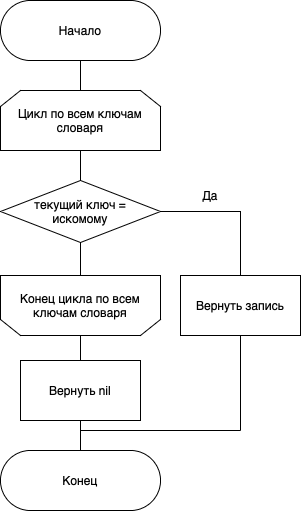
\includegraphics[scale=1]{default.png}
    \caption{Алгоритм поиска методом полного перебора}
    \label{img:default}
\end{figure}

\begin{figure}[H]
    \centering
    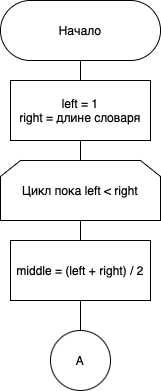
\includegraphics[scale=1]{bin_1.png}
    \label{img:bin_1}
\end{figure}

\begin{figure}[H]
    \centering
    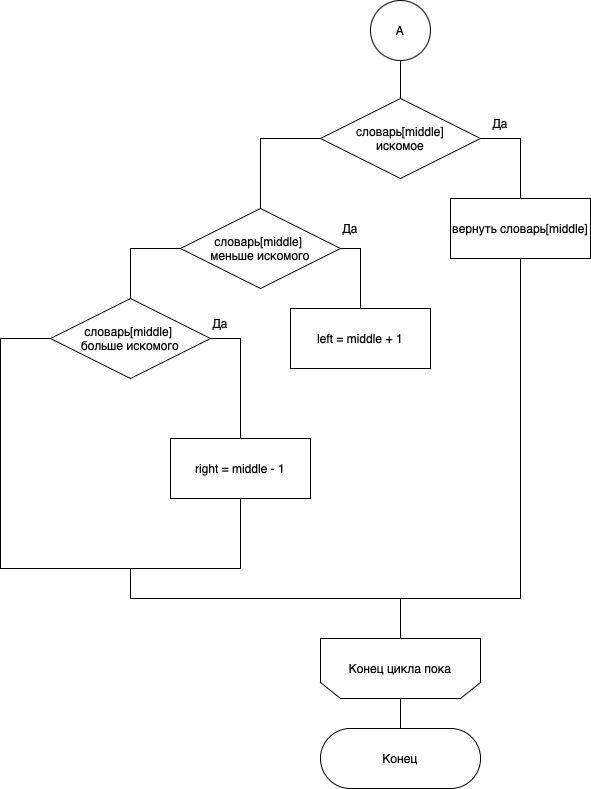
\includegraphics[scale=0.8]{bin_2.png}
    \caption{Алгоритм поиска методом дихотомии}
    \label{img:bin_1}
\end{figure}

\begin{figure}[H]
    \centering
    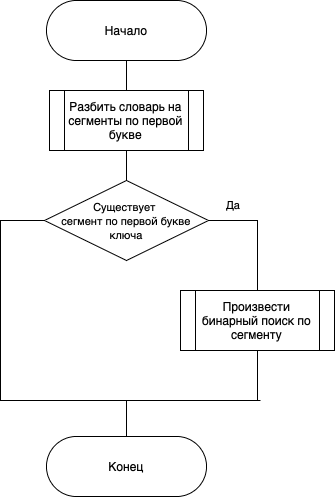
\includegraphics[scale=1]{seg.png}
    \caption{Алгоритм поиска методом частотного анализа}
    \label{img:seg}
\end{figure}

\subsection{Описание структуры программного обеспечения}

На рисунке \ref{img:uml} представлена \textit{uml} диаграмма разрабатываемого программного обеспечения.

\begin{figure}[H]
    \centering
    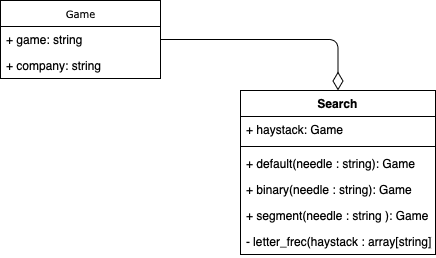
\includegraphics[scale=1]{uml.png}
    \caption{Структура программного обеспечения}
    \label{img:uml}
\end{figure}

\subsection{Описание используемых типов данных}

При реализации алгоритмов будут использованы следующие структуры данных:

\begin{itemize}
    \item ключ --- строка;
    \item словарь --- двумерный массив строк.
\end{itemize}

\subsection{Структура программного обеспечения}

Программное обеспечение состоит из следующих модулей:

\begin{itemize}
    \item main.lua --- модуль, содержащий код точки входа;
    \item search.lua --- модуль, содержащий код функций поиска;
    \item type.lua --- модуль, содержащий объявление словаря;
    \item benchmark.lua --- модуль, содержащий функции замера временных характеристик.
\end{itemize}

\subsection{Тестирование}

Тестирование будет проводиться методом черный ящик. В таблице \ref{tab:tests} представлены тесты. \\

\begin{table}[H]
    \caption{Тестирование представленных реализаций алгоритмом поиска по словарю}
    \centering
    \begin{tabular}{|c|c|c|}
    \hline
    Ввод              & Ожидаемый результат                & Фактический результат              \\ \hline
    qop               & qop Quiet River                    & qop Quiet River                    \\ \hline
    theHunter Classic & theHunter Classic Expansive Worlds & theHunter Classic Expansive Worlds \\ \hline
    Dota 3            & Не найдено                         & Не найдено                         \\ \hline
    \end{tabular}
    \label{tab:tests}
\end{table}

\subsection{Вывод}

В данном разделе были представлены схемы алгоритмов, структура по, типы данных, тесты.

\section{Технологическая часть}

В данном разделе приведены средства реализации и листинги кода.

\subsection{Средства реализации}

К языку программирования выдвигаются следующие требования:

\begin{enumerate}
    \item Возможность производить замер времени выполнения части программы.
    \item Существуют среды разработки для этого языка.
    \item Возможность чтение из файла, запись в файл, создание массивов.
\end{enumerate}

По этим требованиям был выбран язык Lua.

\subsection{Листинги кода}


\begin{lstlisting}[caption=Словарь, label=list:matrix, language={}]
Game = {}

Game.__index = Game

function Game:New(n, c)
    assert(n ~= nil and c ~= nil, 'name and company must be provided')
    
    local self = setmetatable({}, Game)
    
    self.game = n
    self.company = c

    return self
end

function Game:__tostring()
    return self.game .. " : " .. self.company 
end
    
return Game
\end{lstlisting}

\begin{lstlisting}[caption=Точка входа, label=list:matrix, language={}]
local s = require 'split'
local csv = require 'csv'
local game = require 'type'
local search = require 'search'
local bench = require 'benchmark'
local cmp = require 'cmp_count'

function main()
    data, err = csv.read('../data/data1.csv', ';')

    local dict = {}

    for i, v in ipairs(data) do
        local g = Game:New(v[1], v[2])

        table.insert(dict, g)
    end

    io.write("Ipnut game name: ")
    local g_name = io.stdin:read('l')

    io.write('Benchmark? (y/n): ')

    local y_n_debug = io.stdin:read('l')
    local finder = search:New(dict)

    if y_n_debug == 'y' then
        local res = total_cmp(dict)

        dump_cmps(res, '../data/cmps.csv')

        print(string.format("Default: %f", bench.cpu_run(function ()
            finder:default(g_name)
        end, 1000, 'ns')))
        print(string.format("Binary:  %f", bench.cpu_run(function ()
            finder:binary(g_name)
        end, 1000, 'ns')))
        print(string.format("Segment: %f", bench.cpu_run(function ()
            finder:segment(g_name)
        end, 1000, 'ns')))
    else
        local sd = finder:default(g_name) or 'not found'
        local sb = finder:binary(g_name)  or 'not found'
        local ss = finder:segment(g_name) or 'not found'

        print('Default:', sd[1], sd[2])
        print('Binary: ', sb[1], sb[2])
        print('Segment:', ss[1], ss[2])
    end
end

main()
\end{lstlisting}

\begin{lstlisting}[caption=Реализация алгоритмов поиска, label=list:matrix, language={}]
local search = {}
search.__index = search

function search:New(h)
    local self = setmetatable({}, search)

    self.haystack = h
    self.segments = nil

    return self
end

function search:default(needle)
    local haystack = self.haystack

    local comp = 0

    for i, v in ipairs(haystack) do
        comp = comp + 1
        if v.game == needle then
            return {v, comp}
        end
    end

    return {nil, comp}
end

function search:binary(needle)
    local haystack = self.haystack
    local left = 1
    local right = #haystack

    local comp = 0

    while left <= right do
        local middle = math.floor((left + right) / 2)

        if (haystack[middle].game == needle) then
            comp = comp + 1
            return {haystack[middle], comp}
        elseif haystack[middle].game < needle then
            comp = comp + 2
            left = middle + 1
        else
            comp = comp + 2
            right = middle - 1
        end
    end

    return {nil, comp}
end

local function letter_freq(haystack)
    local res = {}

    for i, v in ipairs(haystack) do
        if res[v.game:sub(1, 1)] == nil then
            res[v.game:sub(1, 1)] = { v }
        else
            table.insert(res[v.game:sub(1, 1)], v)
        end
    end

    return res
end

function search:segment(needle)
    local haystack = self.haystack

    if self.segments == nil then
        self.segments = letter_freq(haystack)
    end

    local letter = needle:sub(1, 1)
    local cmp = 0
    for k, v in pairs(self.segments) do
        cmp = cmp + 1
        if k == letter then
            local value = search:New(v)
            local res = value:binary(needle)
            
            res[2] = res[2] + cmp
            return res
        end
    end

    return nil
end

return search
\end{lstlisting}

\subsection{Вывод}

В данном разделе были разработаны алгоритмы поиска.

\section{Исследовательский раздел}

В данном разделе будет проведен замер временных характеристик выполнения алгоритмов и пример работы программы.

\subsection{Пример работы программы}

На рисунке \ref{img:ex} представлен пример запуска программы. \\

\begin{figure}[H]
    \centering
    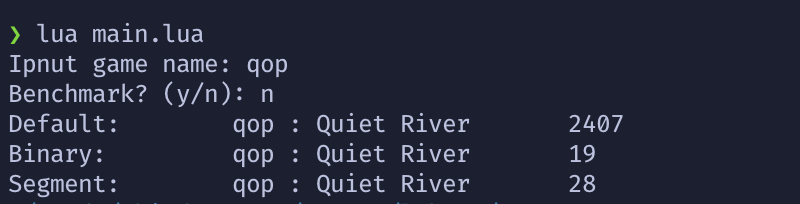
\includegraphics[scale=1.2]{ex.png}
    \caption{Пример работы программы}
    \label{img:ex}
\end{figure}

\subsection{Технические характеристики}

Технические характеристики электронно-вычислительной машины, на которой выполнялось тестирование:

\begin{itemize}
    \item операционная система: macOS BigSur версия 11.4;
    \item оперативная память: 8 гигабайт LPDDR4;
    \item процессор: Apple M1.
\end{itemize}

\subsection{Временные характеристики}

В данном работе более интересующей нас характеристикой будет являться количество сравнений, необходимое для нахождения ключа, так как от количества сравнений прямо пропорционально зависит время работы алгоритма. Количество элементов в словаре примерно 2500.

Поиск будет проводиться с помощью каждого реализованного алгоритма, после чего будут представлены соответствующие графики. В каждом построенном графике данные будут отсортированы по возрастанию, так как количество сравнений для алгоритмов, не использующих полный перебор, количество сравнений будет являться "случайной" величиной.

\subsubsection{Алгоритм полного перебора}

\begin{figure}[H]
    \centering
    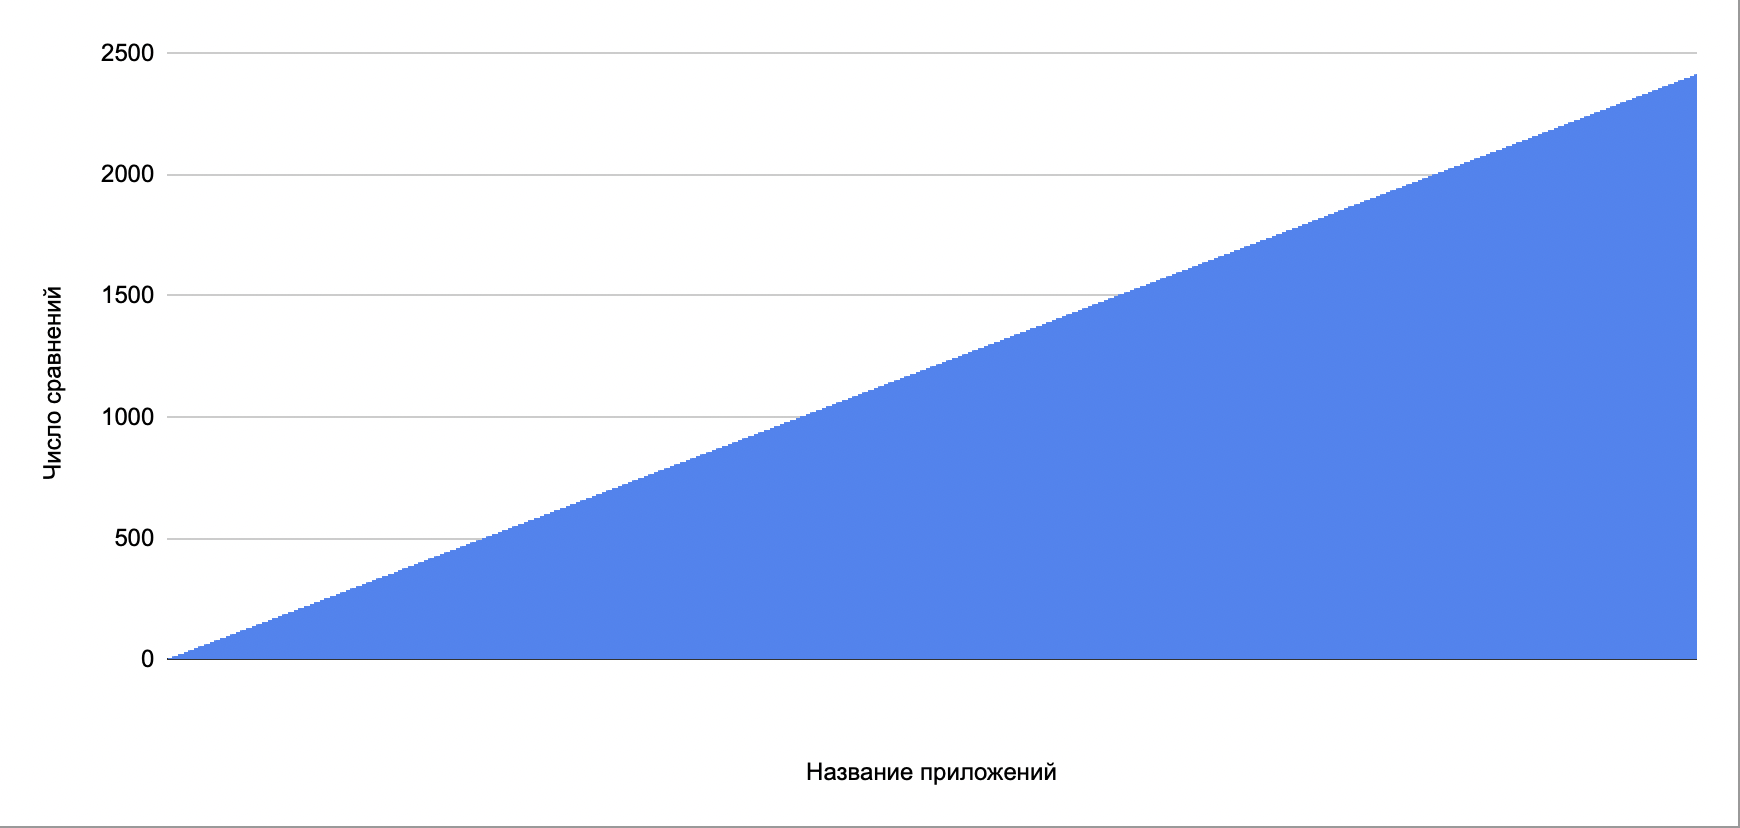
\includegraphics[scale=0.55]{plot_def.png}
    \caption{График количества сравнений для алгоритма поиска полным перебором}
    \label{img:plot_def}
\end{figure}

Как видно из графика \ref{img:plot_def} количество сравнений линейно зависит количества элементов в словаре. Лучшим случаем для алгоритма полного перебора будет являться нахождение искомого элемента в самом начале словаря, тогда как худшим будет являться элемент, находящийся в самом конце словаря.

\subsubsection{Алгоритм бинарного поиска}

\begin{figure}[H]
    \centering
    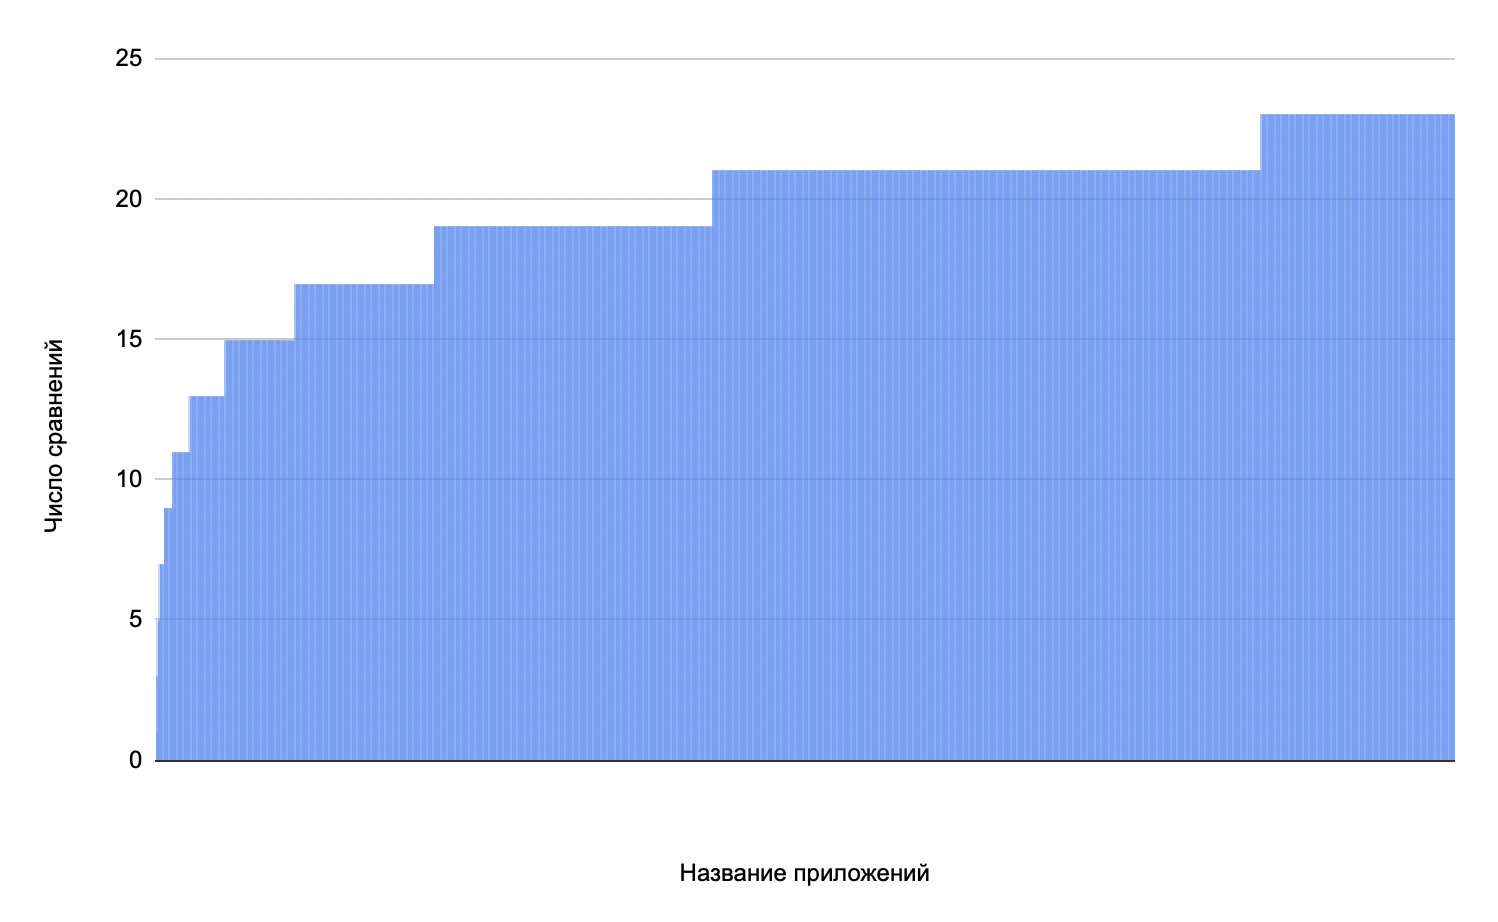
\includegraphics[scale=0.55]{plot_bin.png}
    \caption{График количества сравнений для алгоритма поиска методом дихотомии (данные в графике отсортированы по возрастанию)}
    \label{img:plot_bin}
\end{figure}

Как видно из графика \ref{img:plot_bin} минимальное количество сравнений равно 1 (элемент находится ровно по середине), а максимальное равно 23. По сравнению с последовательным алгоритмом среднее количество сравнений отличается примерно в 61 раз.

\subsubsection{Алгоритм частотного анализа}

\begin{figure}[H]
    \centering
    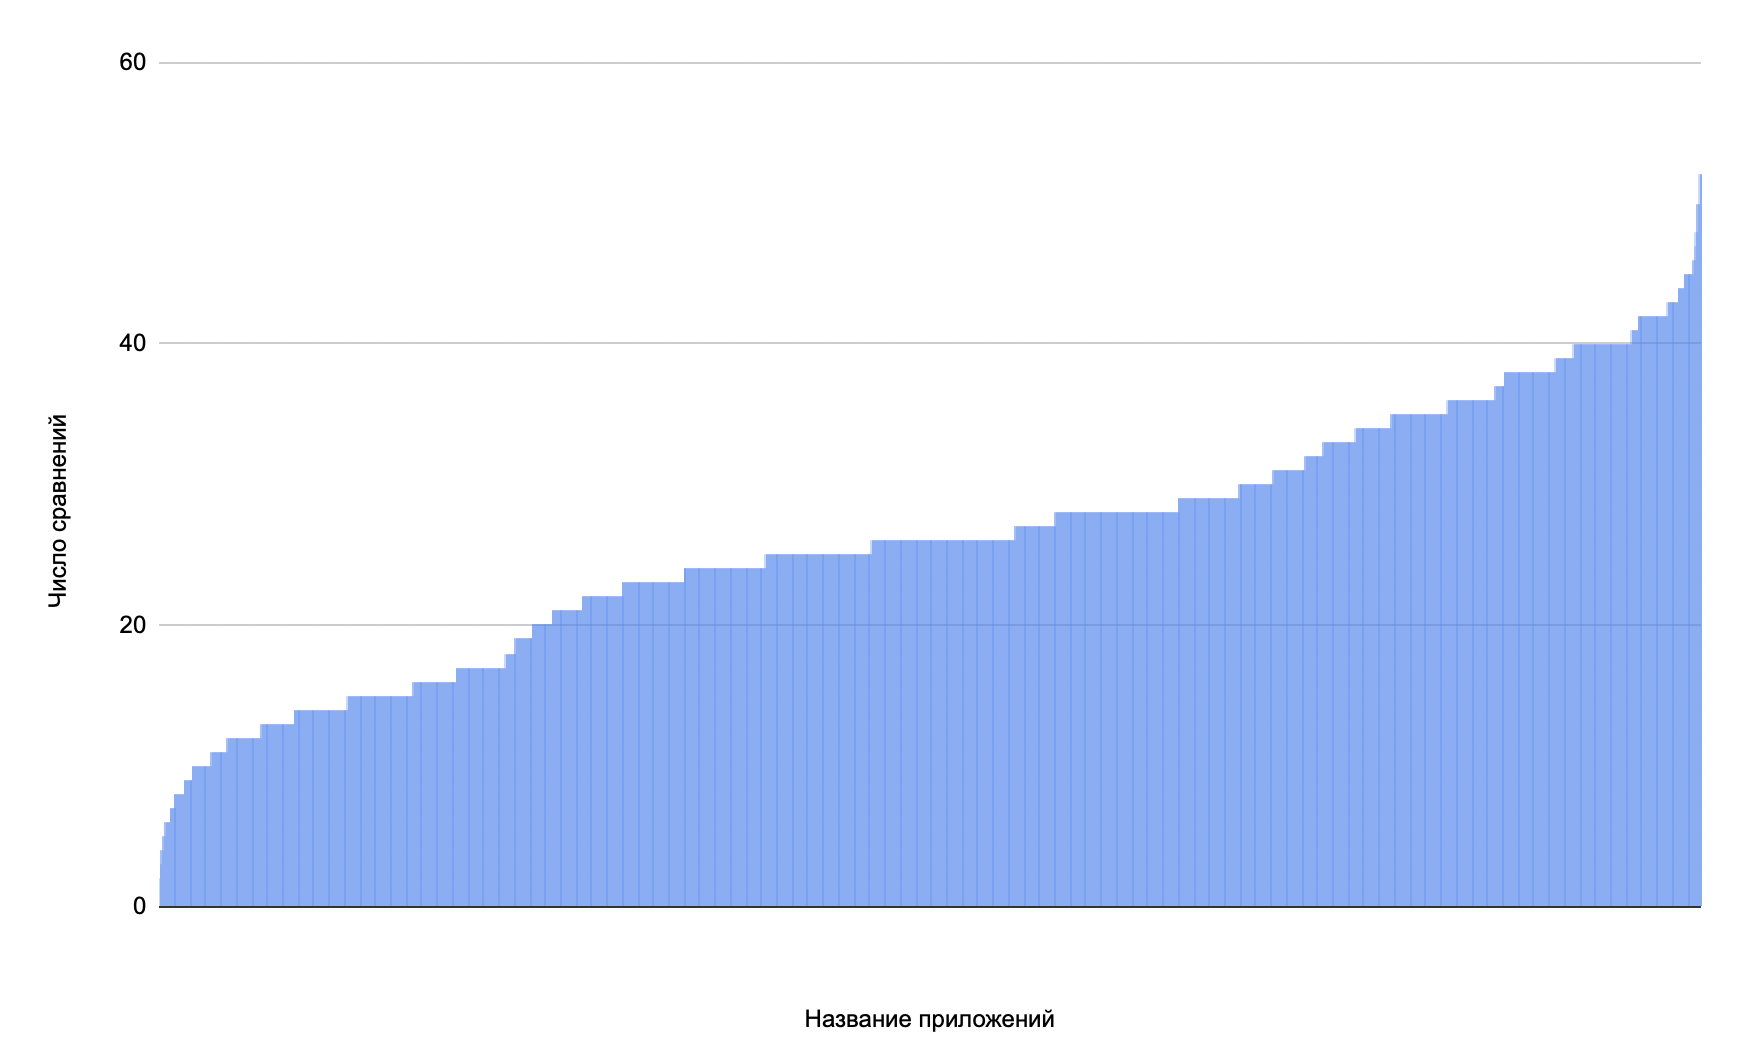
\includegraphics[scale=0.55]{plot_seg.png}
    \caption{График количества сравнений для алгоритма частотного анализа (данные в графике отсортированы по возрастанию)}
    \label{img:plot_seg}
\end{figure}

Так как словарь содержит не только буквы латинского словаря, то в худшем случае потребуется пройти по всему списку алфавита начальных букв словаря, что может потребовать значительное количество сравнений.

На рисунке \ref{img:plot_seg} видно, что в лучшем случае потребуется 2 сравнения (элемент находится по середине первого сегмента). В худшем же 52 сравнения. В среднем количество сравнений в алгоритме полного перебора и алгоритме частотного анализа отличаются в 46 раз. Но по сравнению с алгоритмом бинарного поиска в 1.36 сравнений больше.

\subsection{Вывод}

Исходя из вышеперечисленных данных, можно сделать вывод, что наиболее эффективным алгоритмом поиска является бинарный алгоритм. Алгоритм частотного анализа же лишь в особых случаях будет быстрее бинарного поиска (если алфавит будет сильно ограничен и размер словаря будет очень большим), так как требуется произвести сегментацию словаря, что требует значительное количество времени.

Отдельно стоит отметить, что бинарному поиску требуется подавать на вход отсортированный словарь, на что может потребоваться значительное количество времени и в единичных случаях поиска последовательный алгоритм может быть эффективнее. Но если требуется произвести серию поисков, то время, затраченное на сортировку словаря, окупится сниженным временем поиска.

\anonsection{Заключение}

В данном лабораторной работе были изучены алгоритмы поиска по словарю.

Среди рассмотренных алгоритмов наиболее эффективным оказался алгоритм бинарного поиска.

В рамках данной работы была выполнена цель и решены следующие задачи:

\begin{enumerate}
    \item Изучены алгоритмы поиска по словарю.
    \item Протестированы алгоритмы поиска по словарю.
    \item Замерено и сравнено количество сравнений алгоритмов.
    \item Сделаны выводы на основе проделанной работы.
\end{enumerate}

\anonsection{Список литературы}

\begin{enumerate}
    \item Visual Studio Code [Электронный ресурс], режим доступа: https://code.visualstudio.com/ (дата обращения: \today)
	\item LPDDR4 [Электронный ресурс] \url{https://ru.wikipedia.org/wiki/LPDDR#LPDDR4} (дата обращения: \today)
	\item Ульянов М. В. Ресурсно-эффективные компьютерные алгоритмы. Разработка и Анализ. - Наука Физматлит, 2007. - 376.
	\item Язык Lua. [Электронный ресурс] Режим доступа: https://www.lua.org (дата обращения: \today)
	\item Вирт Н. Алгоритмы + структуры данных = программы. — М.: «Мир», 1985. — С. 28.
\end{enumerate}

\end{document}
